\label{overview}

\section{Overview of the Tool}

CSAtool is a simulation environment based on capacitive network models tailored on each specific DAC topology. These models are based on vectors and matrix that reproduce the circuit proerties of a DAC topology. Given few parameters, among which the most important is the desired value of the unit capacitor ( the smallest compact capacitive element of the DAC), the tool produce a realization of a desired topology and evaluate its performance. In general the tool does NOT provide dedicated models of capacitors (MiMcaps, MoMcaps, PiPcaps...), but allows the designer to customize all the parameters which are necessary to model any of these options.

The main window of the tool, depicted in figure \ref{fig:main} presents the following sections:

\begin{figure}[h!]
	\centering
	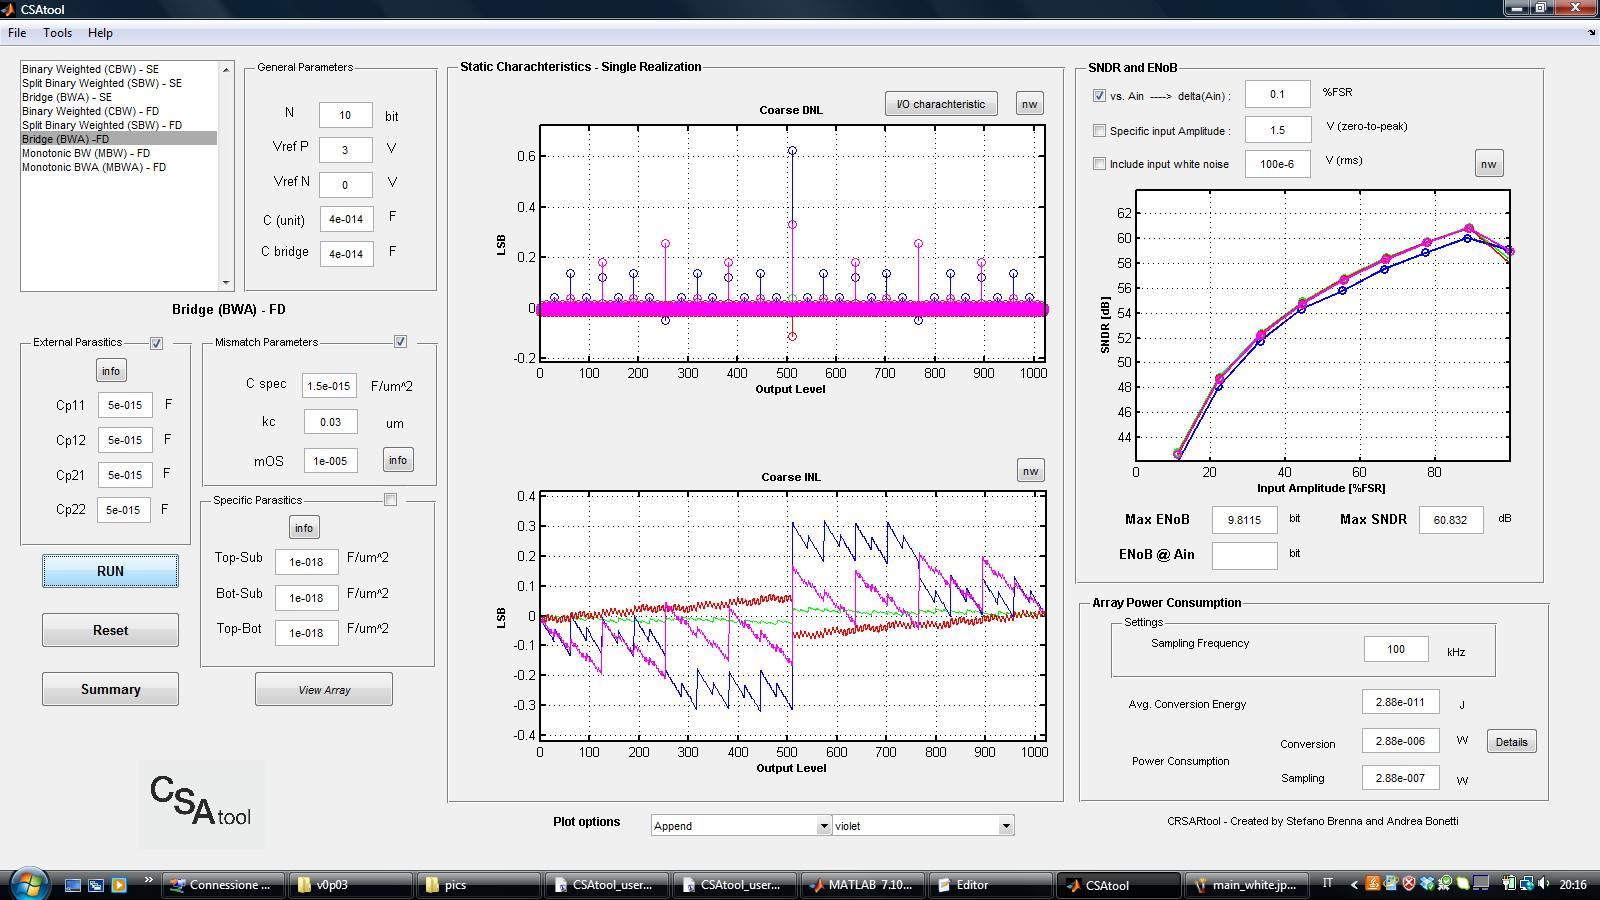
\includegraphics[scale=0.35]{pics/main_white.jpg}
	\caption{CSAtool main window.}
	\label{fig:main}
\end{figure}


\begin{description}

	\item[Topology] \hfill \\
	The topology of the CSAtool can be selected here among a list of the most common ones, at the top-left corner of the GUI main window. Both the array structure and the used switching scheme determine the topology. In addition, it is possible to choose either the single-ended (SE) or the fully-differential (FD) version. \\ The implemented models allow to choose among the following topologies:

\begin{itemize}
\item \texttt{Classic Binary Weighted - CBW (SE and FD)}: traditional binary weighted array combined to a traditional switching algorithm.
\item \texttt{Split Binary Weighted - SBW (SE and FD)}: binary weighted array where the MSB capacitor is split into a replica of the remaining part of the DAC, combined to the split capacitor array switching algorithm.
\item \texttt{Binary Weighted with Attenuation Capacitor BWA (SE and FD)}: simmetrical binary weighted array with attenuation capacitor combined to a traditional switching algorithm.
\item \texttt{Monotonic Binary Weighted MBW (intrinsically FD)}: traditional binary weighted array combined to a monotonic switching algorithm.
\item \texttt{Monotonic Binary Weighted with Attenuation Capacitor - MBWA (intrinsically FD)}: simmetrical binary weighted array with attenuation capacitor combined to a monotonic switching algorithm 
\end{itemize}

For additional information on the topologies and the switching schemes briefly described above, please refer to the papers listed in the section \emph{CSAtool Topologies References}.

	\item[General Parameters] \hfill \\
	General parameters section is located to the right of the topology selection list. The number of bits (N) , the input voltage range (difference between $V_{ref,P}$ and $V_{ref,N}$) and the nominal size of  the unit $C_{u}$ and the eventual attenuation capacitor $C_{b}$ can be arbitrarily set here. 

	\item[Mismatch Parameters] \hfill \\
          Each element of the capacitive DAC can be defined as the sum of its nominal value, which is a power of 2 multiple of the unit element, a mismatch contribution and the related parasitic. To contain the mismatch, in real DACs each capacitive bank of the array is typically implemented as the parallel of a desired number of unit capacitors.
 For this reason the mismatch contribution is here expressed and modeled as the sum of the mismatch of each unit element. Mismatch is absumed to be normally distributed with a zero-mean and a standard deviation which depends on the Pelgrom coefficient $k_{c}$ and the specific capacitance $C_{spec}$.

	The parameter \texttt{Cspec} is specific capacitance and it is defined as follows:
\begin{equation}
	C_{spec} = {C \over {W_{C} L_{C}}}
\end{equation}
\noindent Where $W_{C}$ and $L_{C}$ are respectively the width and the length of the unit capacitor whose value is $C$. Moreover, the parameter \texttt{kc} can be obtained from the following equation:
\begin{equation}
	\sigma \left ({\Delta C \over C} \right ) = k_{C} \sqrt{W_{C} L_{C}} + m_{OS}
\end{equation}
\noindent Where $\sigma \left ({\Delta C \over C} \right )$ is the standard deviation of the difference $\Delta C$ of identically designed capacitors, normalized to their absolute value $C$. The parameter $m_{OS}$ is given by the technology.
To enable the mismatch effect estimation, the checkbox related section of the main window must be checked.
\begin{figure}[h!]
	\centering
	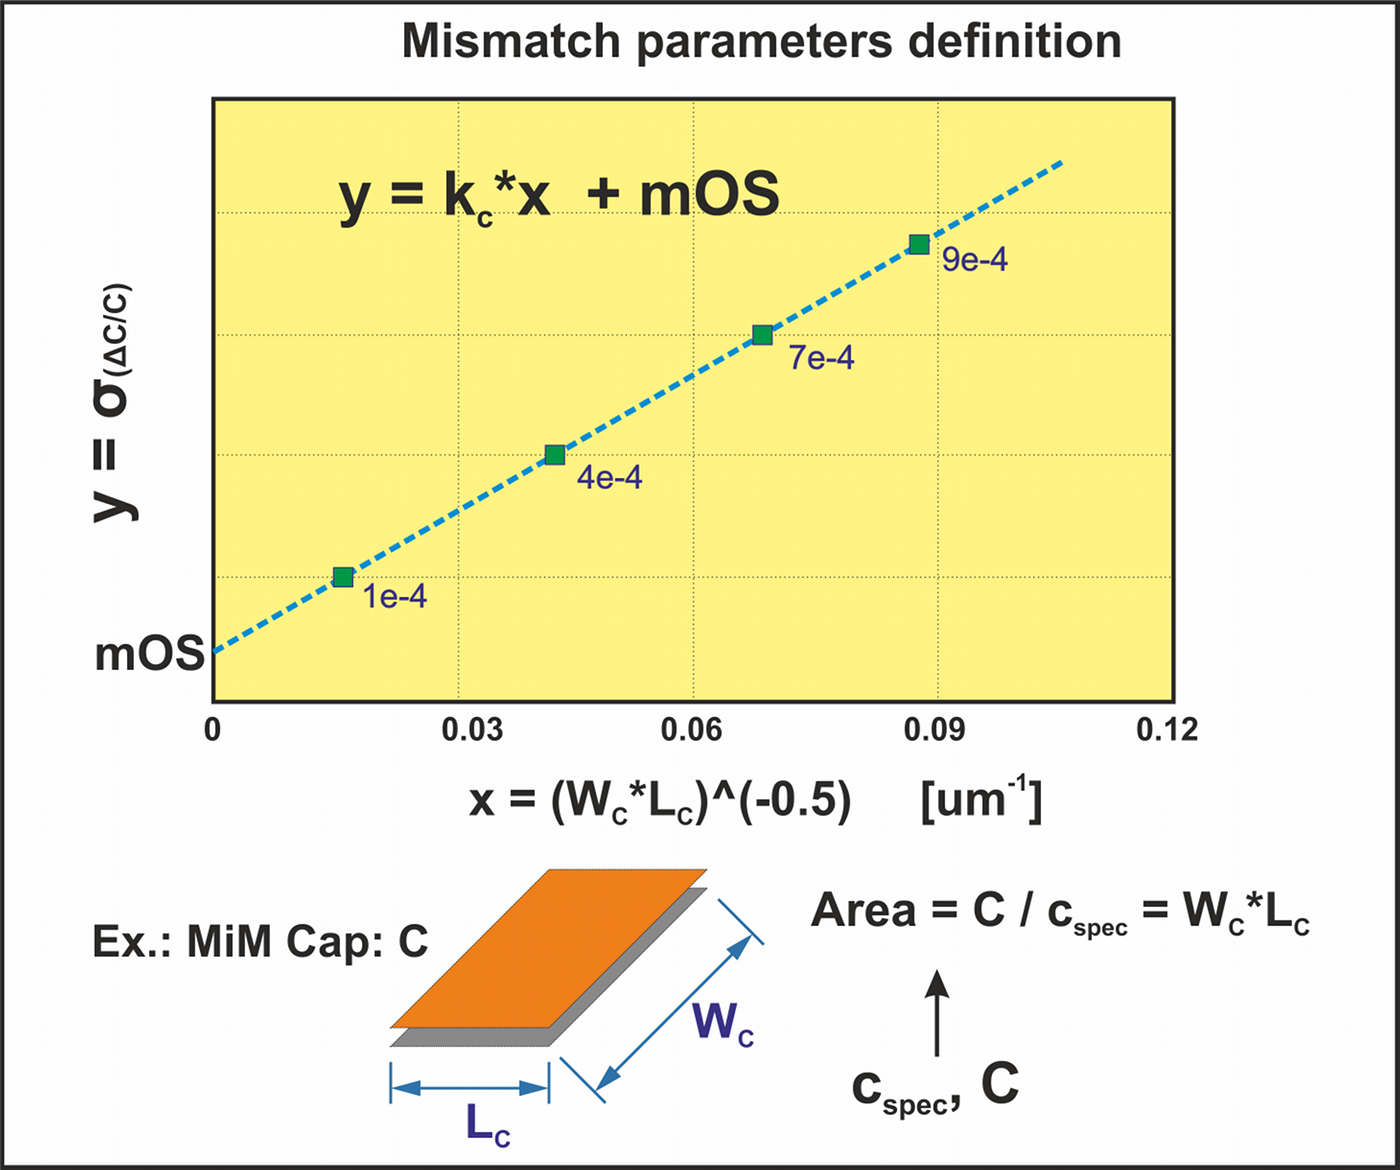
\includegraphics[scale=0.8]{pics/mismatch.png}
	\caption{Definition of the parameters for the mismatch of the capacitors.}
	\label{fig:mismatch}
\end{figure}

\item[Intrinsic Parasitics] \hfill \\
           It is possible to add the values of  intrinsic parasitic capacitances that are connected from the top-plate of the designed array (or sub-arrays) to the substrate, and from the the top-plate to the bottom-plate of every unit capacitor used to compose each capacitive bank of the DAC. The area-dependent parasitic capacitances to specify are the ones connected from the top plate of the capacitor to the substrate (Top-Sub), from the bottom plate of the capacitor to the substrate (Bot-Sub) and from the top plate to the bottom plate of the capacitor (Top-Bot).
This functionality is provided to give the designer the chance to evaluate the impact of those parasitics which are intrinsic of a particular class of capacitor and depend on its area, which is fixed by its size and specific capacitance.

\begin{figure}[h!]
	\centering
	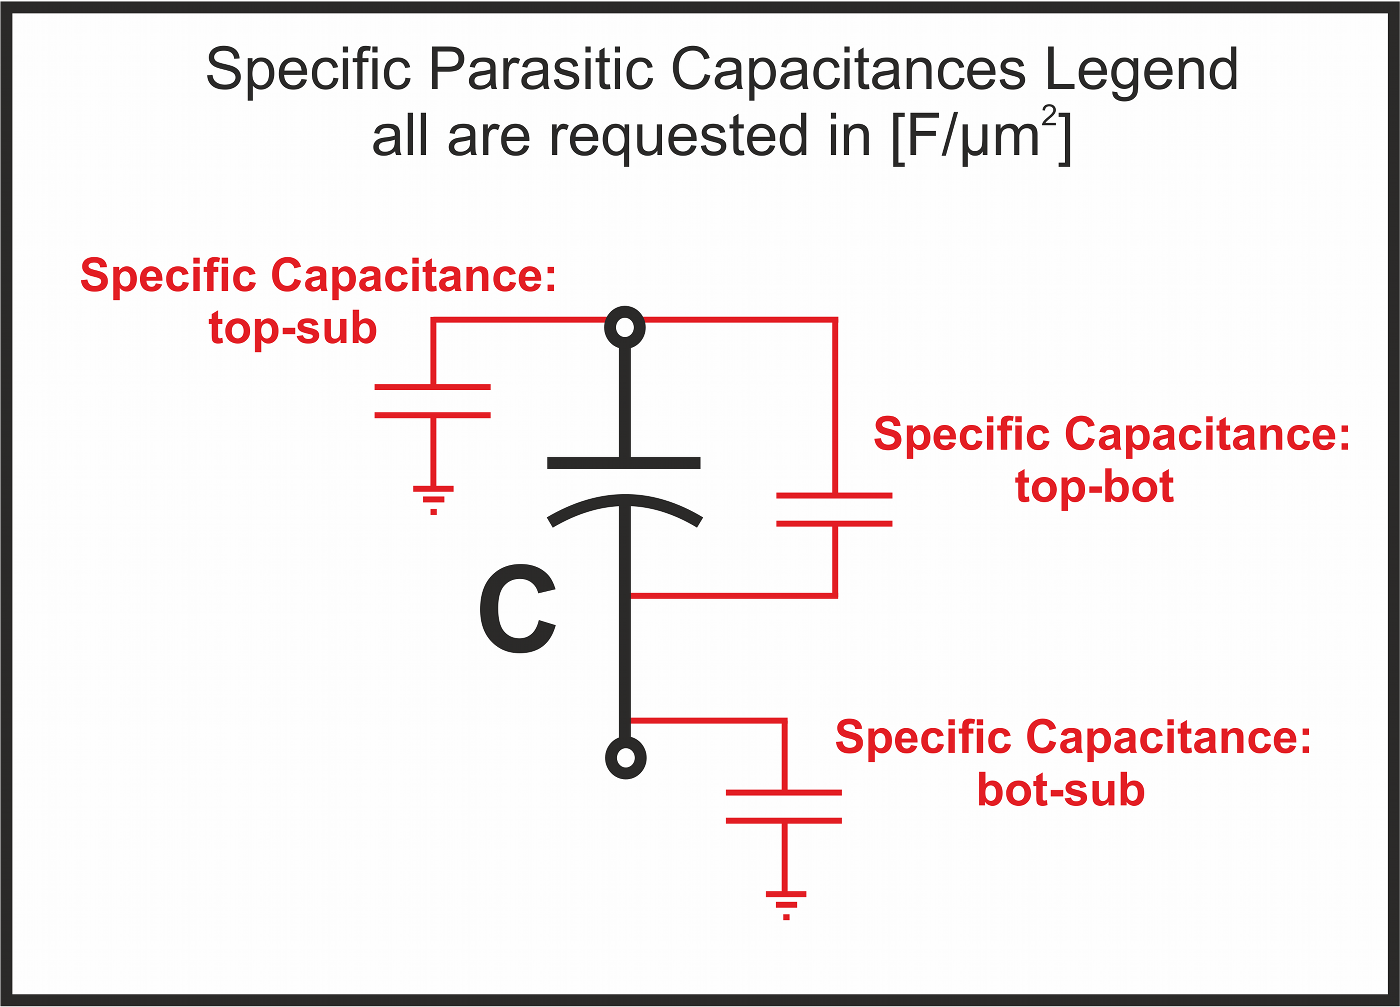
\includegraphics[scale=0.5]{pics/specpar.png}
	\caption{Specific parasitic capacitances.}
	\label{fig:specpar}
\end{figure}

Once again, it is worth noting here that in general the tool does NOT provide dedicated models of capacitors (MiMcaps, MoMcaps, PiPcaps...), but allows the designer to customize all the parameters which are necessary to model them. To enable the intrinsic parasitic effect estimation, the checkbox related section of the main window must be checked.

	\item[External Parasitics] \hfill \\
	The values of the external parasitic capacitances affecting the top plate node of DAC can be added here. The parasitic capacitances to specify are the ones connected from the top plate of the capacitive DAC and eventual sub-DACs to the substrate or to any fixed voltage node (for example $VDD$, $VSS$ or $V_{ref,P}$ and $V_{ref,N}$, if they don't coincide).\texttt{Cp11},\texttt{Cp12},\texttt{Cp21} and \texttt{Cp22} are the values that can be set in the most general case, depicted in figure \ref{fig:viewcpar}. If you have any doubt about the nodes affected by these parasitics, you can press the \texttt{View Array} button: an illustration will help you. 
	
\begin{figure}[h!]
	\centering
	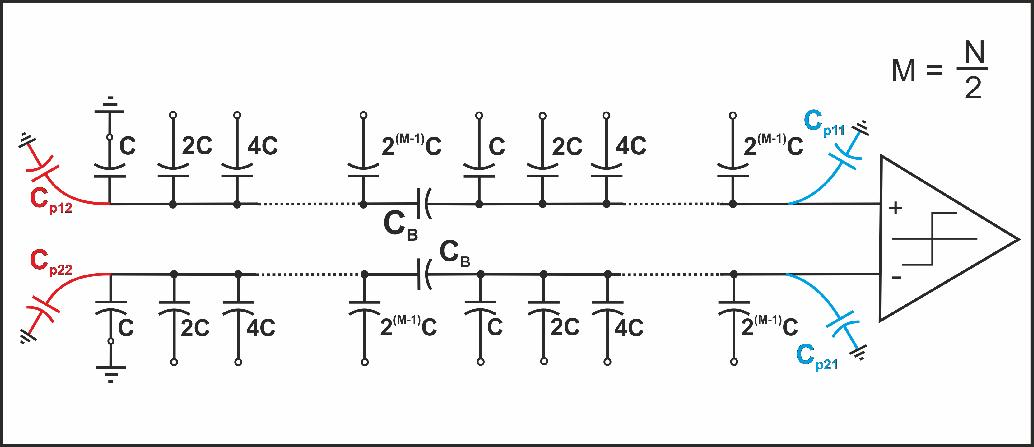
\includegraphics[scale=0.35]{pics/viewpar.jpg}
	\caption{External parasitic capacitances for a fully differential BWA.}
	\label{fig:viewcpar}
\end{figure}
	
To enable the external parasitic effect estimation, the checkbox related section of the main window must be checked.

	\item[Static Characteristics - Single Realization] \hfill \\
	Both DNL and INL graphs of the ADC are shown here for a single realization, estimated each time you press the \texttt{Run} button. By selecting the \emph{append} plot option, successive realizations can be compared on the same graph. 

	\item[SNDR and ENoB] \hfill \\
	The dependency of the SNDR on the amplitude of the input signal is plotted here, in the top right section of the main window. 
To enable this estimation, you can check any of the first two box on the top left. The first box allows to evaluate the SNDR of the customized DAC by points as a function of the input amplitude. The amplitude has a fixed step set by the user in the \texttt{delta(Ain)} cell and expressed as fraction of the FSR (i.e. 0.1 means 10 points). Both maximum achievable ENoB and SNDR are reported. \\
Differently, the second box enables the evaluation of the ENoB at a given input amplitude.
To estimate the dynamic performance, the tools simulate a conversion of an input sinusoid sampled well over nyquist, according to the IO charachteristic of the converter, including the current realization mismatch and  parasitics. The FFT is then performed on the output to evaluate the desired spectral metrics.
This approach also allows to sum a desired input referred white noise, defined by its rms value. This option just models an input referred noise and do not deal directly with its possible sources (comparator, switches...).

\begin{figure}[h!]
	\centering
	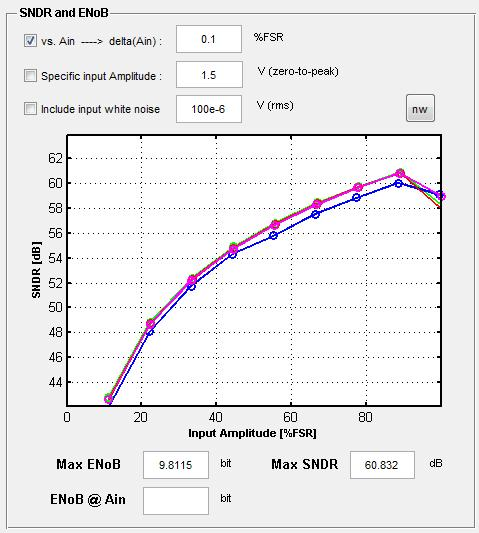
\includegraphics[scale=0.65]{pics/dynamic.jpg}
	\caption{Dynamic metrics estimation section.}
	\label{fig:dynamic}
\end{figure}

	\item[Array Power Consumption] \hfill \\
	By setting the sampling frequency of the ADC, it is possible to estimate the average energy required per conversion. The power consumptions of the conversion and of the sampling phase are also reported and include the impact of parasitics. \\ \textbf{This functionality is currently under development and could result  inaccurate for fully differential topologies.}
	
\end{description}